\documentclass{article}
\usepackage{graphicx}
\usepackage{fullpage}
\usepackage{hyperref}
\usepackage{caption}
\usepackage{subcaption}
\usepackage{tikz}

%\usepackage{fontspec}
%\setmainfont{Times New Roman}

\begin{document}

\title{NDN MOG Project Snapshot}
\author{Zening Qu}
\maketitle

\abstract
To be filled.

\tableofcontents
\listoffigures
\listoftables
\newpage

%-------------------------------------------------------------------------------------------------------------------------------------%
% Introduction
%-------------------------------------------------------------------------------------------------------------------------------------%
\section{Introduction: Objective, Inspiration and Potential Findings}
\label{itro}
%Massively Multiplayer Online Games (MMOGs) are gaining research attention these years. The LPP project is an exploration of the design and creation of such games on Named Data Network (NDN). The {consistency}, scalability, availability and security issues of MMOG design are of special interest. As of genre and gameplay, we are interested in creating an Role Playing Game (RPG) inspired by \emph{Le Petit Prince}, which is how this project got its name.

%This document is a snapshot of the current progress of the LPP project. It is aimed for the research group to reflect on the finished work and plan the next steps. It contains an in-progress survey of MMOG design issues in the IP world (section \ref{bg}), a brief description of our previous NDN car racing game (section \ref{prew}) and designs of LPP which is our logical next step (section \ref{nstp}). 

% Define the document, Intended readers
This document is aimed for the Named Data Networking Multiplayer Online Game (NDN MOG) research group. It is written at a time when a small scale car racing game was implemented and synchronized on the NDN testbed \cite{egalcar}. The author tries to provide a rich background of MOG design, in the hope of fostering the design and evaluation of a more extensive Role Playing Game (RPG) game over NDN. The author does not attempt to bring up too much details about NDN. Interested readers should turn to the project website (\href{http://www.named-data.net/}{http://www.named-data.net/}) and its publication list.

%subject to change as we write on
In this section we define the project objective and potential findings. Section \ref{ggd} introduces the general game design of our planned RPG game and compares it with characteristics of World of Warcraft (WoW), the representative MOG. The MOG synchronization problem and related design issues are described in section \ref{dfsync}. Finally, section \ref{dslpp} tries to solve the synchronization problem for our RPG game and evaluate the solution. Note that NDN MOG is an on-going project, hence section \ref{dslpp} is merely a best-effort solution for the time being. The document may raise more questions than it answers. Its content (including background and design) is subject to substantial improvement and change.

\subsection{Project Objective: Explore The Game Synchronization Problem And The Related Problems}
The primary objective is to explore the game synchronization problem on NDN. Closely related problems such as architecture choice, interactivity and scalability are seriously considered. Other related problems like availability and security are taken into account whenever possible. These problems are depicted in section \ref{dfsync}.

%\subsection{Project Inspiration: P2P MOGs In The IP World}
%In the industry, the Client/Server (C/S) architecture dominant the MOG world. Large MOGs, or Massively Multiplayer Online Games (MMOGs) like World of Warcraft use clusters of servers to handle its thousands of players despite the high cost, service bottleneck and single point-of-failure brought by the centralized servers \cite{Neumann07, Fan10}. 

%In the academia, there has been debate about P2P architecture's potential for MOGs and MMOGs. Some researchers are very pessimistic: in 2010, Miller et al. predicted that MMOGs with WoW-like scale cannot be deployed using the available P2P scheme \cite{Miller10}. Other researchers find the future of P2P support for MMOGs attractive: in 2004 Knutsson et al. simulated a P2P MOG which scaled up to 4,000 concurrent players \cite{Knutsson04}, and many other P2P schemes were proposed after that \cite{Fan10}. Many researchers agree that the common future of P2P and MMOG remains promising, but for P2P architectures to be a practical alternative of the C/S architecture, many challenges persist: consistency, interactivity, scalability, availability, security etc. \cite{Neumann07, Fan10, Gilmore12}. 

%P2P game synchronization problem is closely related to these challenges that lay ahead (see section \ref{dfsync}). If the synchronization problem is better solved, P2P MOGs are likely to experience a performance increase. Given NDN's many characteristics such as intrinsic multicasting \cite{Jndn}, there is a potential that NDN can provide better support for P2P MMOGs than IP does (see section \ref{dslpp}).

\subsection{Potential Findings: Impact of NDN On P2P MOGs}
% subject to change
Potential findings of the project include but are not limited to:
\begin{itemize}
\item A prototype RPG game on NDN, with synchronized game state
\item An evaluation of the design of the game, regarding consistency, latency, scalability etc.
\item A library/toolkit that supports the proposed mechanism
\end{itemize}



%-------------------------------------------------------------------------------------------------------------------------------------%
% MMOGs and our Gameplay
%-------------------------------------------------------------------------------------------------------------------------------------%
\section{General Game Design: LPP and WoW}
\label{ggd}
In this section we present general game design of our prototype RPG game \emph{LPP} (inspired by \emph{Le Petit Prince}) and compare it with the representative MMOG World of Warcraft (WoW). We do not intend to create a game of similar complexity in terms of gameplay, but we hope to simulate interactions that are typical in WoW and find out the game's scalability. In this way, our experiment will carry more practical value.

\subsection{Genre: Role Playing Game}
Role-playing games (RPG) is the genre we want to study. Most existing MMOGs, like WoW, are RPGs \cite{Knutsson04}. These games allow thousands of concurrent players to interact in a shared game world, which poses a big challenge in network bandwidth. Although other game genres such as real-time strategy (RTS) games and first-person shooter (FPS) games also supports massive concurrent users, these games are often divided into small isolated sessions where a small group of players communicate exclusively within the group \cite{Knutsson04}. Therefore RTS games and FPS games present smaller challenges to the network and are not studied in this project.

\subsection{Scale: 1 Million Concurrent Players}
WoW is the world's most subscribed MMORPG. It has more than 10 million subscribers in worldwide \cite{wow12, Schiano11}. In 2008 its number of concurrent players was reported to reach a peak value of 1 million \cite{wow08}. 

%We are interested in the scalability problem because (1) it is one of the major challenges faced by P2P MMOGs and (2) it is directly influenced by the synchronization problem (see \ref{dfsync}). While maintaining game state consistency, we hope to scale our game up. The scale of WoW should act as a reminder of MMOG requirements from the industry.

\subsection{Activities: Raiding and PvP}
\label{sec:act}
In most MMOGs, the base map, or the land, is immutable. Players experience the virtual world through sensibilities of their avatars. In \cite{Suznjevic08, Suznjevic09}, the authors performed an action-specific analysis of WoW's network traffic and proposed the following taxonomy of game activities:
\begin{itemize}
\item Questing: avatars interact with non-player characters (NPCs) in the virtual world.
\item Dungeons: a small group of five avatars work together to kill a series of more powerful NPCs; each group is isolated from other groups and players; replications of dungeons are instantiated for each group.
\item Raiding: the same as Dungeons, except that NPCs are more powerful and group size is larger (10, 25 or 40).
\item Trading: trade of goods between players or between a player and an NPC.
\item PvP: player versus player combat; number of participants can reach 80.
\end{itemize}
Figure \ref{act} reports characteristics of different types of activities. Among the five action types Raiding and PvP combat involves the largest number of players, requires most cooperation and communication (figure \ref{actstar}). Consequently, these two types have the highest requirement in bandwidth and latency (figure \ref{actbw} and \ref{actltc}). Because Raiding and PvP combat are so challenging, they deserve serious consideration in our experiment. We emphasis these two forms of activities in the design of our prototype game (see section \ref{lppgp}).

\begin{figure}
\begin{center}
\begin{subfigure}[b]{\textwidth}
	\begin{center}
	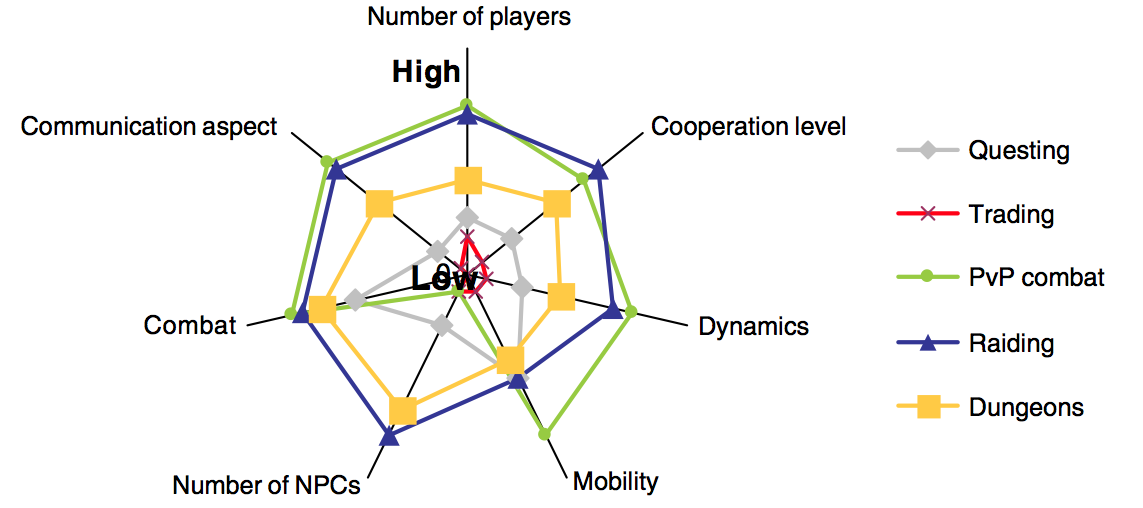
\includegraphics[scale=0.3]{images/actstar.png}
	\caption{An overall comparison of various action types. Note that Raiding and PvP combat have higher requirements in multiple dimensions, which may lead to greater challenges to the network.}
	\label{actstar}
	\end{center}
\end{subfigure}
\begin{subfigure}[b]{\textwidth}
	\begin{center}
	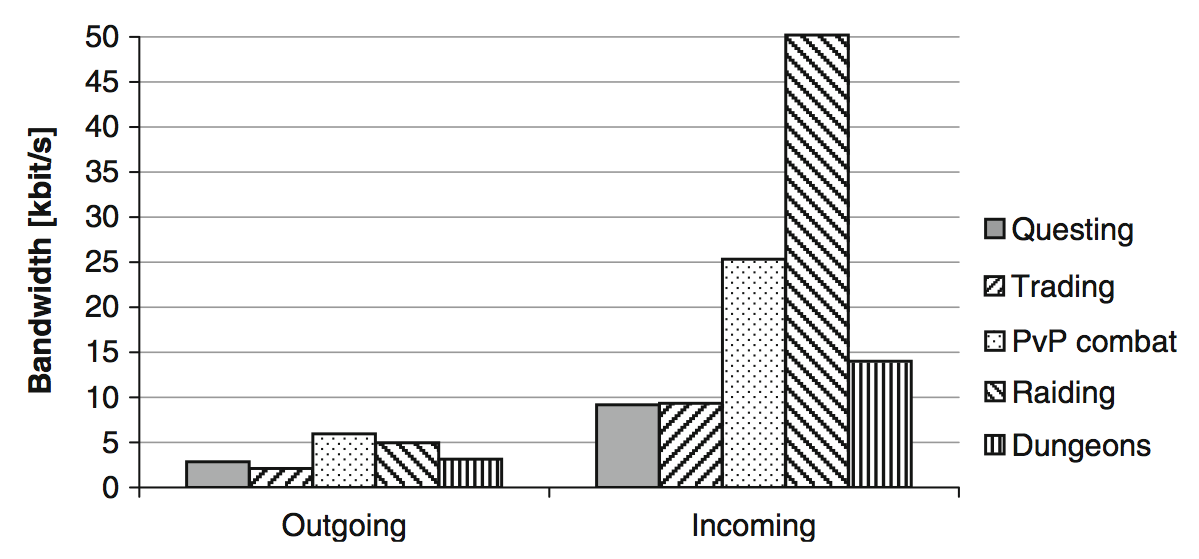
\includegraphics[scale=0.25]{images/actbw.png}
	\caption{Bandwidth requirement of action types. The label "Outgoing" means traffic from the client to the server. The label "Incoming" means traffic from the server to the client. Traffic is measured at the client's side. Node that Raiding and PvP combat consume much more bandwidth than the other action types.}
	\label{actbw}
	\end{center}
\end{subfigure}
\begin{subfigure}[b]{\textwidth}
	\begin{center}
	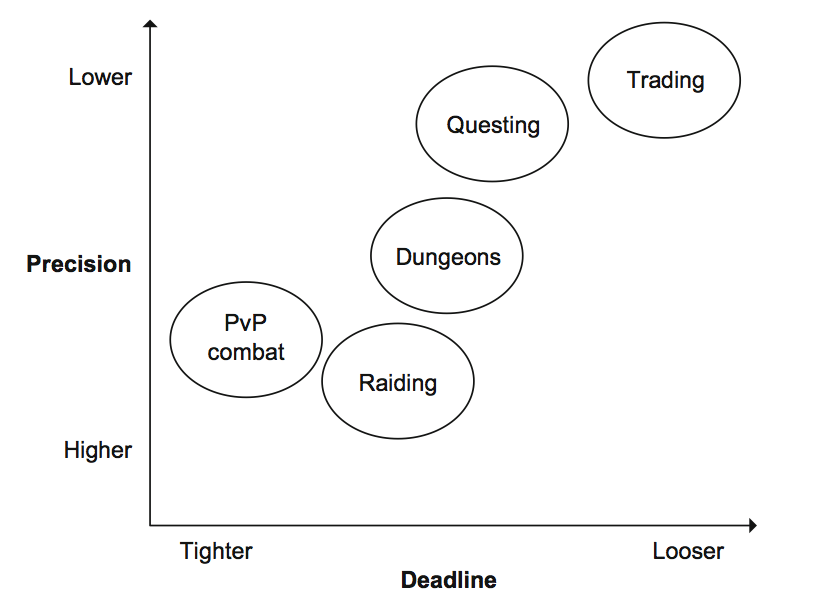
\includegraphics[scale=0.3]{images/actltc.png}
	\caption{Latency requirement of action types. Raiding and PvP combat have the highest requirement in both precision and latency. This means that players actions should be more precise in terms of spatial accuracy when involved in these two activities, and they are given less time to perform these actions. In these scenarios, network latency is an especially sensitive issue.}
	\label{actltc}
	\end{center}
\end{subfigure}
\caption{Player actions evaluated under various metrics. All three graphs excerpted from \cite{Suznjevic09}}
\label{act}
\end{center}
\end{figure}


\subsection{LPP Gameplay}
\label{lppgp}
Our prototype RPG is inspired by Antoine de Saint-Exup\'ery's novel \emph{Le Petit Prince}, which is how it got the name LPP. The novel is about a young and innocent alien prince who left his home planet for a long journey. He traveled to several asteroids and planets and witnessed many people and things that he considers absurd or ``adult-like''. During his stay on the earth, he met a fox who told him:``It is the time you have wasted for your rose that makes your rose so important.'' He tamed the fox, and the fox became unique and important to him. His experience and wisdom grew on this journey.

As mentioned in section \ref{sec:act}, we are primarily interested in player actions similar to Raiding and PvP combat in WoW. Hence the LPP gameplay lies follows:
\begin{itemize}
\item Players take up the role of the prince.
\item The game dynamically instantiates foxes, which are NPCs.
\item Players try to tame foxes using spells. This corresponds to Questing in WoW.
\item Players can form large groups to tame foxes. This corresponds to Raiding in WoW.
\item Players combat with each other to practice their skills in casting a spell. This corresponds to PvP combat in WoW.
\item As players tame foxes and practices with each other, their wisdom, or experience, grow.
\end{itemize}


%-------------------------------------------------------------------------------------------------------------------------------------%
% The Sync Problem
%-------------------------------------------------------------------------------------------------------------------------------------%
\section{The Synchronization Problem and Related Problems}
\label{dfsync}
This section tries to shed light on the MOG synchronization problem and its related problems by providing information from the literature. We summarized that the goal of the synchronization problem is to reach game state consistency (section \ref{sec:cm}) and explained why architecture choice, interactivity and scalability are closely related to the synchronization problem (section \ref{sec:rp}).

\subsection{Consistency Models: Event Based (P2P) and Update Based (C/S)}
\label{sec:cm}
% the graph: fully connected P2P model, obviously not scalable (latency is great, but the bandwidth requirement is too high)
% If you want it to scale, you will have to trade great latency for scale
% but you will need a mechanism to limit the latency, like Knutsson did in 2004
Thousands of players experience a shared virtual world in a MMOG. Media of the virtual world (such as 3D models of the land, buildings, NPCs and characters) and the \emph{game logic} (rules of how this world should function and how its members should interact) are typically installed on the player's machine. In addition to that every player needs a copy of the \emph{game state} in order to learn the evolvement of the world. The game state is the state of the virtual world plus the state of all participating players, NPCs and objects. It is obvious that the game state changes as time passes by. Players interact with the world by generating actions that changes the game state. Because each player has a replication of the game state, a consistency issue arises: copies of game state should always be consistent with each other or else players' opinions of the virtual world would diverge. Researchers have proposed various models and algorithms to ensure such consistency.

Two consistency models exists: event-based and update-based (see figure \ref{fig:cm}) \cite{Gilmore12}. The event-based consistency model is used on fully distributed P2P networks where every peer is directly connected to \emph{all other peers}. Each peer maintains a replication of the global game state and send \emph{event}s that represent the player's action in the virtual world to all other peers. As newer global game state can only be computed when the game logic has sufficient input, i.e. actions of all relevant peers within a relevant time period, each peer actively listens to events published by all other peers. Moreover, due to the uncertainty of transmission delay events may arrive at a peer out of their generation order. Peers need a synchronization algorithm to figure out the generation order of received events in order to compute the correct game state. Common synchronization algorithms are time warp algorithm \cite{Fujimoto99}, trailing state algorithm \cite{Cronin04}, time bucket algorithm \cite{Gautier98, Diot99} and their variations. These algorithms are discussed in section \ref{sec:sa}.
Note that a peer could also use a reliable, ordered delivery service to make sure it receives all events and in the right order. Yet it is reported that such services would significantly degrade game performance \cite{Fgame}, and are rarely adopted. % double-check this

The update-based consistency model is used on C/S MOGs. Clients do not inter-connect with each other but communicate through a central server. Clients also do not have the right to compute the global game state -- this is withhold by the server. As illustrated in figure \ref{fig:cm}b, clients merely generate events according to player actions and wait for \emph{update}s of the global game state computed by the server. Clients then applie the update to its local game state. Depending on the lower layer services used by the client and server, a client may need to occasionally reorder its received updates. The central server also need a synchronization algorithm to process all received events in their generation order. The synchronization algorithms here are identical to those in the event-based sync model.
% so, no matter what architecture it is, the sync algorithms are the same! I didn't know this before!

\begin{figure}
\begin{center}
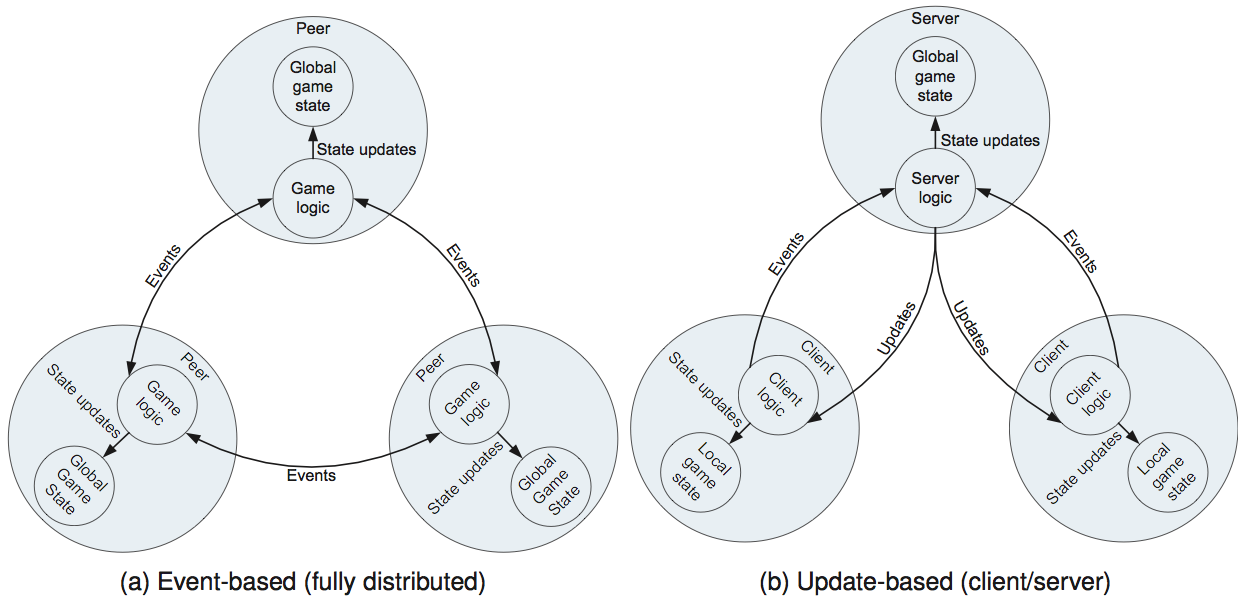
\includegraphics[scale=0.3]{images/sm.png}
\caption{Consistency Models. Excerpted from \cite{Gilmore12}}
\label{fig:cm}
\end{center}
\end{figure}

\subsection{Synchronization Algorithms: Conservative and Optimistic}
\label{sec:sa}
As previously mentioned, both event-based and update-based consistency models need synchronization algorithms (see section \ref{sec:cm}). In other words, both P2P MOGs and C/S MOGs need synchronization algorithms.

The game synchronization problem can be described as follows. Machine A is running a game sync algorithm. It is connected to some other machines. These machines share the same set of data. The data set does not grow but its value changes in a fast pace. All machines that are connected to A may request to update the data set but only A has the authority perform the update. So A has to gather all requests and know their relative order, otherwise the value of the data set would be wrong. In a C/S architecture, this machine A would be the server (figure \ref{fig:archcs}). It would gather client events and publish game updates. In a P2P architecture, this machine A could be any peer (figure \ref{fig:archp2p}), as every peer holds the right to update a certain subset of the global game state. In a hybrid architecture (see section \ref{sec:arch}), this machine A would be one of the cluster servers (figure \ref{fig:archhbr}). It would gather requests from both its clients and its peer cluster servers.

Note that game synchronization problems differs from sync algorithms for other applications (such as file syncing) in that (1) the content to be synced does not grow in size, but changes instead (2) the time constraint is much more tight. Such difference is reflected in the design of game sync algorithms, which emphasis on packet ordering and network latency.

Both conservative and optimistic synchronization algorithms have been proposed. Conservative algorithms are based on lockstep. Arrived events are delayed until it is safe to process them. Optimistic algorithms process arrived events once they are received, but performs game state rollbacks once it receives an event that arrives late. A simulation-based evaluation of these algorithms is shown in figure \ref{fig:sa}, from which we can see that optimistic sync algorithms outperform conservative ones (figure \ref{fig:saclm}). 

In \cite{Ferretti05} the author proposed an algorithm to further improve optimistic sync performance by exploiting game semantics. The author exploited the ``correlation'' among received events and effectively reduced rollback ratios, thus enhancing performance (figure \ref{fig:sapct}). Similar strategy should be used in the LPP project (see section \ref{sec:dslpp}).

\begin{figure}
\begin{subfigure}[b]{0.3\textwidth}
\begin{center}
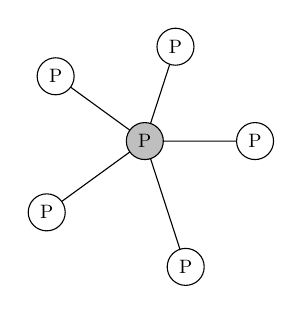
\begin{tikzpicture} [scale=0.7, transform shape]
\tikzstyle{every node}=[draw,shape=circle];
\node [fill = gray!50] (v0) at (0:0) {P};
\node (v1) at ( 0:2) {P};
\node (v2) at ( 72:1.8) {P};
\node (v3) at (2*72:2) {P};
\node (v4) at (3*72:2.2) {P};
\node (v5) at (4*72:2.4) {P};
\draw (v0) -- (v1) % star
(v0) -- (v2)
(v0) -- (v3)
(v0) -- (v4)
(v0) -- (v5);
\end{tikzpicture}
\end{center}
\caption{P2P}
\label{fig:archp2p}
\end{subfigure}
%
\begin{subfigure}[b]{0.3\textwidth}
\begin{center}
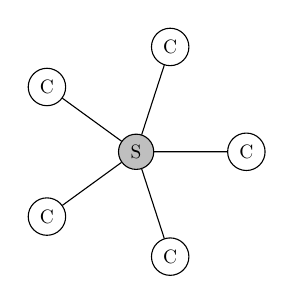
\begin{tikzpicture} [scale=0.7, transform shape]
\tikzstyle{every node}=[draw,shape=circle];
\node [fill = gray!50] (v0) at (0:0) {S};
\node (v1) at ( 0:2) {C};
\node (v2) at ( 72:2) {C};
\node (v3) at (2*72:2) {C};
\node (v4) at (3*72:2) {C};
\node (v5) at (4*72:2) {C};
\draw (v0) -- (v1) % star
(v0) -- (v2)
(v0) -- (v3)
(v0) -- (v4)
(v0) -- (v5);
\end{tikzpicture}
\end{center}
\caption{C/S}
\label{fig:archcs}
\end{subfigure}
%
\begin{subfigure}[b]{0.3\textwidth}
\begin{center}
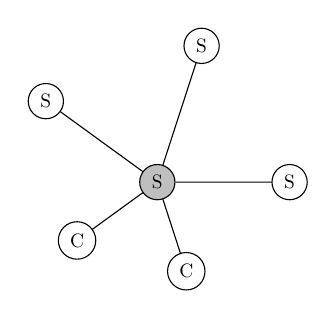
\begin{tikzpicture} [scale=0.7, transform shape]
\tikzstyle{every node}=[draw,shape=circle];
\node [fill = gray!50] (v0) at (0:0) {S};
\node (v1) at ( 0:2.4) {S};
\node (v2) at ( 72:2.6) {S};
\node (v3) at (2*72:2.5) {S};
\node (v4) at (3*72:1.8) {C};
\node (v5) at (4*72:1.7) {C};
\draw (v0) -- (v1) % star
(v0) -- (v2)
(v0) -- (v3)
(v0) -- (v4)
(v0) -- (v5);
\end{tikzpicture}
\end{center}
\caption{Hybrid}
\label{fig:archhbr}
\end{subfigure}
\caption{Synchronization in different architectures. C stands for client. S stands for server. P stands for peer. The shaded node represents the node that is running a game synchronization algorithm.}
\label{fig:arch}
\end{figure}

\begin{figure}
\begin{center}
\begin{subfigure}[b]{\textwidth}
	\begin{center}
	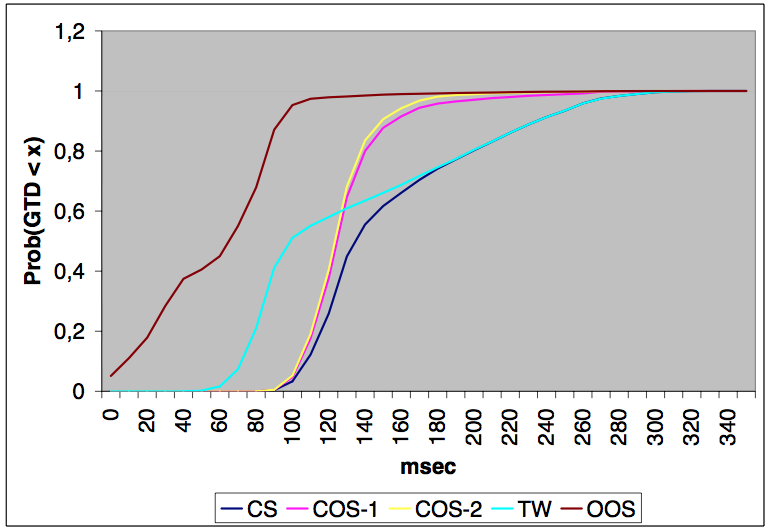
\includegraphics[scale=0.3]{images/saclm.png}
	\caption{Cumulative probability of packets' arrival. The vertical axis is the cumulative probability. The horizontal axis is the elapsed time. The quicker an algorithm reaches 1, the smaller latency it has. The tolerate threshold is 150ms according to the author of the graph.}
	\label{fig:saclm}
	\end{center}
\end{subfigure}
\begin{subfigure}[b]{\textwidth}
	\begin{center}
	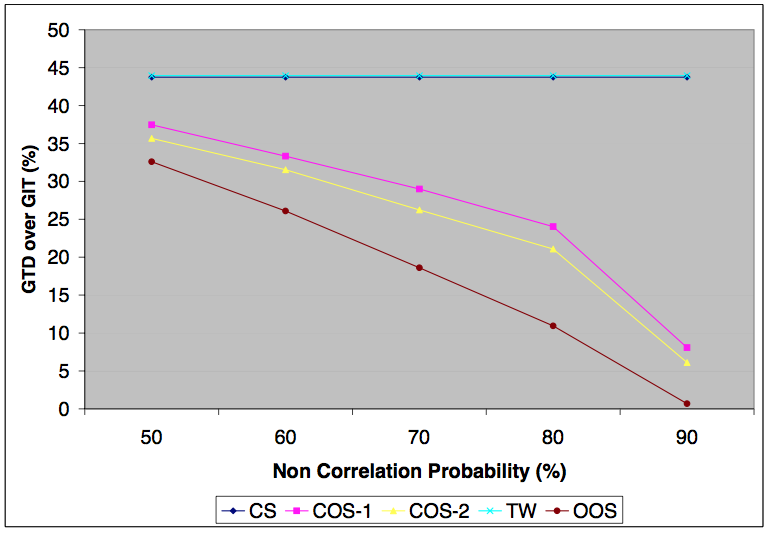
\includegraphics[scale=0.3]{images/sapct.png}
	\caption{Percentage of packets with intolerable latency (more than 150ms). The vertical axis is the percentage. The horizontal axis is the ``non correlation probability'' of successive events. Large values would mean that the received events are less correlated, which would incur less rollbacks and consequently faster processing (note that the latency here includes the time spent in rollbacks).}
	\label{fig:sapct}
	\end{center}
\end{subfigure}
\caption{Latency of various synchronization algorithms. CS stands for conservative synchronization. TW stands for time warp, which is representative of optimistic sync algorithms. OOS is a variation of time warp which was proposed by the author of \cite{Ferretti05}. COS-1, COS-2 are CS variations. Both graphs are excerpted from the same paper.}
\label{fig:sa}
\end{center}
\end{figure}


\subsection{Related Problems: Architecture, Interactivity, Scalability, Availability, Security}
\label{sec:rp}

\subsubsection{Architecture Choice: P2P, C/S, Hybrid}
\label{sec:arch}
% same sync algorithm but on different architectures, will the effect be the same?

\subsubsection{Interactivity: MMOGs are Latency-Sensitive}
% the interactivity threshold: 100~150ms
% latency comprises of transmission delay and synchronization delay

\subsubsection{Scalability: P2P Is Scalable, But Not Traditional P2P Consistency Model}
% bandwidth requirement
% I think P2P requires more bandwidth than C/S does, because the central server gathers information effectively
% to reduce bandwidth requirement, we MUST exploit Locality of Interest

\subsubsection{Availability: Robustness of C/S and P2P}
% P2P is better than C/S, but P2P is not perfect 

\subsubsection{Security: P2P Is More Prone To Cheating}
% P2P is more prone to cheating, but C/S is not ideal either


%-------------------------------------------------------------------------------------------------------------------------------------%
% Design of Our Next Planned Game
%-------------------------------------------------------------------------------------------------------------------------------------%
\section{Designing The Next Game: LPP}
\label{sec:dslpp}

\subsection{Namespace}

\begin{figure}[htbp]
\begin{center}
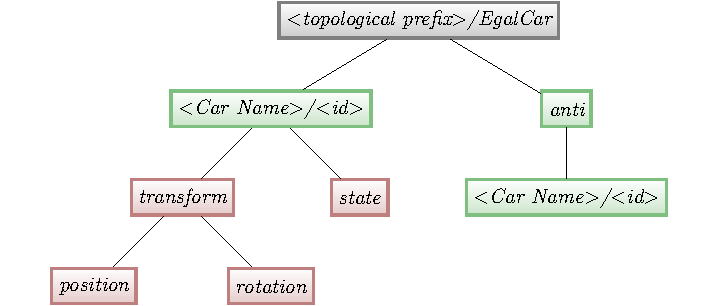
\includegraphics{ObjectTree.pdf}
\caption{Part of LPP's namespace, nodes that contain a ``(sequence number)'' will be explained one by one in this document}
\label{ns}
\end{center}
\end{figure}

\begin{enumerate}
\item \emph{/ndn/ucla.edu/apps/lpp}: the topological prefix of the game
\item \emph{$<$Player ID$>$}: a random number generated in real-time to represent a particular player in the game, this ID is computed in a random manner to (partly) avoid name collisions
\item \emph{$<$Asteroid ID$>$}: a random, real-time number representing a particular asteroid
\item \emph{$<$Seedling ID$>$}: a random, real-time number representing a particular seedling who comes out of a particular asteroid
\item \emph{anti}: this is for asset deletion (publishing an anti-asset corresponds to deleting that particular asset)
\item \emph{.../$<$Player ID$>$/state}: the current state of a particular player; \emph{position} can be used to provide a global view; \emph{experience} can be used to produce a global rank list
\item \emph{.../$<$Asteroid ID$>$/state}: the current state of a particular asteroid, which may contain a name list of all players on that asteroid and things like that
\item \emph{.../$<$Player ID$>$/event}: the action of a particular player
\end{enumerate}

In figure~\ref{ns}, all blue nodes are recognized as \emph{Asset}s, all red nodes \emph{State}s, green ones \emph{Event}s. We will have more documentations about Asset, State, Event in the future. For now it is sufficient to know that these three types of nodes will be synchronized in three different ways.

\subsection{Membership Service and Object Discovery: CCNx Sync}

\subsection{Unreliable, Ordered Delivery of Updates}

\subsection{Reliable, Ordered Delivery of Events}

\subsection{Example of Player-Player Interaction}

\subsection{Example of Player-NPC/Object Interaction}

\subsection{Discussions: Performance}

\bibliographystyle{plain}
\bibliography{MOGRef}
\end{document}